\documentclass[12pt,letterpaper,noanswers]{exam}
\usepackage[usenames,dvipsnames,svgnames,table]{xcolor}
\usepackage[margin=0.9in]{geometry}
\renewcommand{\familydefault}{\sfdefault}
\usepackage{multicol}
\usepackage{wrapfig}
\pagestyle{head}
\definecolor{c03}{HTML}{FFDDDD}
\header{AM 22b Class 02}{}{Jan 27: distance, graphs, contours}
\runningheadrule
\headrule
\usepackage{graphicx} % more modern
\usepackage{amsmath} 
\usepackage{amssymb} 
\usepackage{hyperref}
\usepackage{tcolorbox}

\usepackage[numbered,autolinebreaks,useliterate]{mcode}

\begin{document}
 \pdfpageheight 11in 
  \pdfpagewidth 8.5in

% I need to review the torus trajectories...

\begin{itemize}
    \itemsep0em
    \item Problem set 01 (related to \S 12.1-12.5 of Hughes-Hallett) will be assigned this week, and is due on Thursday Feb 4th.  
    \item Skill checks C02 and C03 are on Monday.  The sample problem for skill check C02 is in this handout.
    \item There is a pre-class assignment due on Monday (it will consist of ~20 minutes of videos, a couple of webwork Qs, and discussion board participation).
\end{itemize}

\hrule
\vspace{0.2cm}

\noindent\textbf{Big picture}

This week we will work with functions of multiple variables as well as with equations in three variables (chapter 12).  The goal is to become familiar with some common functions, equations, and surfaces, to identify correspondences between these, and to be able to interpret information about a function from graphical, analytical, and numerical representations of the information.

\vspace{0.2cm}
\hrule
\vspace{0.2cm}

\noindent\textbf{Skill Check C02 practice}
\begin{questions}
\item Find an expression for the distance between the point $(a,b,c)$ and the plane $y = 7.$

\emph{You'll be given a point and a plane of the form $x = k$ or $y = k$ or $z = k$ where $k$ is a constant).}

\end{questions}


\vspace{0.2cm}

\hrule
\vspace{0.2cm}

\noindent\textbf{Skill Check C02 solution}

Points in the plane are of the form $(x,7,z)$ for any $x,z\in \mathbb{R}$.  

The distance between $(a,b,c)$ and an arbitrary point in the plane is given by \[\sqrt{(a-x)^2 + (b-7)^2 + (c-z)^2}.\]

The distance between the point and the plane is defined as the minimum of all possible distances between the point and a point in the plane.  

$x$ and $z$ are arbitrary, and we choose them so as to find this minimum distance.  $(a-x)^2$ is non-negative, so its minimum is zero (at $x=a$).  Similarly for $(c-z)^2$.  The distance is $\sqrt{(b-7)^2}$.

The distance can be written as $\vert b-7\vert$ or as $\sqrt{(b-7)^2}$.  The expression $b-7$ would not be correct because it may have a negative value.

\vspace{0.2cm}
\hrule
\vspace{0.2cm}

\noindent\textbf{Matlab code example 1}
\begin{lstlisting}
%% Class 02.  Example 01.
% Plot a curve in 2-space (in the xy-plane).
syms x
f = @(x) sin(x*pi/30);
fplot(x,f(x),[0,30],'LineWidth',3)
xlabel('x'); ylabel('y')
title('curve: y = sin(\pi x/30)')
set(gca,'FontSize',10)
% Choose an axis range.
axis equal; axis([0 30 -2 2])
% I adjusted the size of the figure by hand before saving.
print('-opengl','~/Desktop/sinewave.eps','-depsc','-r300')
\end{lstlisting}

\includegraphics[width=\textwidth]{img/sinewave.eps}

\vspace{0.2cm}
\hrule
\vspace{0.2cm}

\noindent\textbf{Matlab code example 2}
\begin{lstlisting}
%% Class 01.  Example 02.
xvals = 0:1:30;
fvals = sin(xvals*pi/30);
plot(xvals,fvals,'-*','LineWidth',3)

% This makes a similar plot.
% It doesn't use the symbolic toolbox.
% It is plotting points (xk,yk) for
% x = 0,1,2,...,30 and
% y = f(0), f(1),...,f(30).

xlabel('x'); ylabel('y')
title('curve: y = sin(\pi x/30)')
set(gca,'FontSize',10)
axis equal
axis([0 30 -2 2])
print('-opengl','~/Desktop/sinewave2.eps','-depsc','-r300')
\end{lstlisting}

\includegraphics[width=\textwidth]{img/sinewave2.eps}

\begin{itemize}
    \item What is the difference between \texttt{\%} and \texttt{\%\%} at the beginning of a line?
    \vspace{1cm}
    
    \item How would you edit this code to plot $(x,f(x))$ values at intervals of $0.2$ in $x$?
    \vspace{0.6cm}
    
    \item How would you edit this code to plot $(x,f(x))$ values at 45 points?
    \vspace{0.6cm}
    
    \item Does \texttt{0:1:30} produce a $1\times 31$ vector or a $31 \times 1$ vector?
     \vspace{0.6cm}
     
\end{itemize}

\vspace{0.2cm}
\hrule
\vspace{0.2cm}

\eject

\noindent\textbf{3-space} (\S 12.1)
\begin{tcolorbox}
A \textbf{coordinate plane} is a plane in $3$-space that contains two axes.  There are three: the $xy$-, $xz$-, and $yz$-planes.  Points of the form $(x,y,0)$, $(x,0,z)$ and $(0,y,z)$, make up the respective planes.

The \textbf{$x$-axis} is made up of points of the form $(x,0,0)$.  This is all points in $3$-space such that $y=0$ and $z=0$.  Similarly for the $y$- and $z$-axes.
\end{tcolorbox}

\vspace{0.2cm}
\hrule
\vspace{0.2cm}

\noindent\textbf{How do you currently think about:}
\begin{itemize}
\itemsep0em
    \item distance
    \item function
    \item domain
    \item image
    \item graph
    \item level set
    \item contour
\end{itemize}

\vspace{0.2cm}
\hrule
\vspace{0.2cm}

\noindent\textbf{Distance} (\S12.1)
\begin{tcolorbox}
The \textbf{distance} between a point $(a,b)$ and a point $(x,y)$ is given by $\sqrt{(a-x)^2+(b-y)^2}$.

The \textbf{distance} between a point $(a,b,c)$ and a point $(x,y,z)$ is given by $\sqrt{(a-x)^2+(b-y)^2+(c-z)^2}$.  You can show this using the Pythagorean theorem.

The \textbf{distance} between a point $(a,b,c)$ and a set of points is the minimum of the distances between that point and each point in the set.
\end{tcolorbox}

Distance is often be used as the basis of an equation in three variables.

\begin{itemize}
    \item The set of all points equidistant to a reference point $(a,b,c)$: \[\sqrt{(x-a)^2+(y-b)^2 + (z-c)^2} = d\] or \[(x-a)^2 + (y-b)^2 + (z-c)^2 = d^2.\]
    \item The set of all points equidistant to the point $(0,0,1)$ and to the plane $z = 3$:
    \[\sqrt{(x-0)^2+(y-0)^2+(z-1)^2} = \sqrt{(x-x_0)^2 + (y-y_0)^2 + (z-3)^2}.\] where points on the plane are $(x_0,y_0,3)$ with $x_0,y_0$ arbitrary.
    
    $\Rightarrow x^2+y^2 + (z-1)^2 = (z-3)^2$. 
    
    $\Rightarrow x^2+y^2 = z^2-9z+9-(z^2-2z+1)$.
    
    
    $\Rightarrow x^2+y^2 = -7z+8$.
\end{itemize}

\begin{tcolorbox}
The set of all points equidistant to a reference point is called a \textbf{sphere}.

The distance to the reference point, $d$, is referred to as the \textbf{radius} of the sphere.

A set of points of the form $z = a(x^2+y^2)+b$ is called a \textbf{paraboloid} (or a \textbf{circular paraboloid}).
\end{tcolorbox}

\vspace{0.2cm}
\hrule
\vspace{0.2cm}


\noindent\textbf{Graphs} (\S 12.2)
\begin{tcolorbox}
% The \textbf{graph} of an equation in three variables, $f(x,y,z) = g(x,y,z)$, is the set of all points $(x,y,z)$ that satisfy the equation.

% The graph of an equation in three variables can often be represented as a surface within $3$-space.

A \textbf{function} $f: X \rightarrow Y$ is a mapping of point in the \textbf{domain} (the set $X$) to points in the \textbf{codomain} (the set $Y$).

The \textbf{image} or $\textbf{range}$ of the function is the set of points $\underline{y} \in Y$ such that $\underline{y} = f(\underline{x})$ for some $\underline{x} \in X$.



The \textbf{graph} of a function $f: X\rightarrow Y$ is the set of all points $(x_1,...x_k,y_1,..,y_n)$ such that $\underline{y} = f(\underline{x})$ for some point $\underline{x} = (x_1,x_2,...,x_k)\in X$ (with $\underline{y} = (y_1,y_2,...,y_n)$.

The \textbf{graph} of a scalar function of two variables,$f:\mathbb{R}^2\rightarrow \mathbb{R}$, is the set of all points $(x,y,z)$ such that $z = f(x,y)$.

The graph of a function of two variables can often be represented as a surface within $3$-space.

% The graph of the equation $y = ax+b$ in $3$-space is the set of points $(x,ax+b,z)$ where $x$ and $z$ are arbitrary.  The graph forms a vertical plane.  The intersection of this plane with a surface is called a \textbf{cross-section} of the surface.
\end{tcolorbox}

\begin{tcolorbox}
In $3$-space, an equation of the form $y = ax +b$ is satisfied by the set of points $(x,ax+b,z)$ where $x$ and $z$ are arbitrary.  These points form a vertical plane in $xyz$-space.  The intersection of such a plane plane with a surface is called a \textbf{cross-section} of the surface.
\end{tcolorbox}

Cross-sections are often used to explore the shape of a surface.
\begin{itemize}
    \item The $y = c$ cross sections of $z = x^2 + y^2$ are given by $\left\{\begin{array}{c} y = c \\ z = x^2 + c^2\end{array}\right.$, so points of the form $(x,c,x^2+c^2)$.  This set of points forms a parabola.
    \item The $x = 2$ cross section of $x^2+y^2+z^2 = 9$ is given by the points in the plane $x=2$ such that $4+y^2+z^2 = 9$ so $\left\{\begin{array}{c} x=2 \\ y^2+z^2 = 5\end{array}\right.$ or $\{(2,y,z): y^2+z^2=5\}$.  This set of points forms a circle.
\end{itemize}
\vspace{0.2cm}
\hrule
\vspace{0.2cm}
\noindent\textbf{Teams}
\begin{multicols}{3}
1.  student names here
\end{multicols}

\vspace{0.2cm}
\hrule
\vspace{0.2cm}

\textbf{Examples}
\begin{enumerate}
    \item Plot $(1,3,4)$ in $3$-space.  \emph{(Add tick marks to the axes)}.
    
    \includegraphics[height=1.5in]{img/C02axes.png}
    \item Compute the distance between $(1,3,4)$ and the $xy$-plane.
    \vspace{0.3in}
    
        \item  Find the distance between $(1,3,4)$ and the plane $x=7$.
        \vspace{0.7in}
        
        \item  Find the distance from $(1,3,4)$ to the $z$-axis.
        \vspace{0.7in}
        
        \item Find the set of points in the intersection of the sphere of radius $3$ centered around $(0,0,4)$ and the plane $z=2$.
        \vspace{1in}
        
        \item Write an equation for the set of points distance $2$ from the point $(1,3,4)$.
        \vspace{0.7in}
        
        \item Write an equation for the set of points distance $3$ from the $z$-axis.
        $(1,3,4)$.
          \vspace{0.7in}
          
\end{enumerate}

\vspace{0.2cm}
\hrule
\vspace{0.2cm}
\noindent\textbf{Contour plots} \S 12.3
\begin{tcolorbox}
%\textbf{For your reference (section 12.3):} \\
For a function $f(\underline{x})$ the set of points $\underline{x}$ such that $f(\underline{x}) = c$ is called the $c$-\textbf{level set} of the function.  Note: the $c$-level set is a set in the domain of $f$.

The $c$-level set for a function of two variables is a set in $2$-space, and is often called a \textbf{level curve} or a \textbf{contour line}.  

If we choose a regular interval, $k$ (called the \textbf{contour interval}), and draw the set of level curves $..., c-k, c, c+k, c+2k, ...$ in the $2$-space, we call the resulting diagram a \textbf{contour diagram}.  Two contour diagrams are shown below.

The $c$-level set for a function of three variables is a set in $3$-space, and is often called a \textbf{level surface}.  



% \emph{production functions}

\end{tcolorbox}




Note: if a point $(x,y)$ is in the $c$-level set, it is not in the (c+1)-level set.  Why not? \\

\noindent\textbf{Examples.}

Mount Greylock, on the left, is the highest point in Massachusetts.

\begin{center}
\includegraphics[width=0.9\linewidth]{img/C03contours.png}
\end{center}


\vspace{0.2cm}
\hrule
\vspace{0.2cm}

\noindent\textbf{Graph vs level set}

In the table below, $x,y,z,w$ are variables.  $c$ is a constant.

\begin{tabular}{|c|c|c|c|c|}
\hline
function & graph & space of graph & level sets & space of level sets\\
\hline
  $y=f(x)$   & set of points $(x,y)$ & curve in $2$-space & $f(x) = c$ & points  in $1$-space\\
   $z=f(x,y)$  & set of points $(x,y,z)$ & surface in $3$-space & $f(x,y) = c$ & curves  in $2$-space\\
   $w=f(x,y,z)$  & set of points $(x,y,z,w)$ & solid in $4$-space & $f(x,y,z)=c$ & surfaces in $3$-space \\
   \hline
\end{tabular}

\vspace{0.2cm}
\hrule
\vspace{0.2cm}

\noindent\textbf{Examples}
\begin{enumerate}
    \item Identify the shape of the contour lines for each of the following functions: 
\begin{itemize}
    \item $f(x,y) = y - x^2$.  Contours are of the form $y - x^2 = c$, so parabolas in $xy$-space.
    \item $f(x,y) = x^2$
    \vspace{0.7cm}
    
    \item $f(x,y) = x^2+2y^2$
       \vspace{0.7cm}
       
    \item $f(x,y) = y^2 - x^2$
       \vspace{0.7cm}
       
\end{itemize}
 



\item  Construct a contour diagram for $f(x,y) = 2x^2 + y^2.$

%\includegraphics{img/C02axes-2.png}

\end{enumerate}

% \textbf{asymptotic}
% \textbf{radial symmetry}
% \textbf{cylinder}
% \textbf{production function}


\vspace{0.2cm}
\hrule
\vspace{0.2cm}







\end{document}